\section{Keypoint Detection}

关键点检测常常应用于特征匹配, 例如在相机校准时, 需要检测棋盘格的角点. 
\subsection{What points are keypoints?}
\begin{itemize}
    \item Repeatablility: 在不同的图像中能够独立找到相同的点.
    \item Saliency: interesting points.
    \item Accuracy: 精确的位置.
    \item Quantity: 有足够多的点.
\end{itemize}

因而我们要求 detector 在光照, 视角, 尺度变化下具有不变性(invariance).

在这里我们主要讨论 Corner Detection.

\subsection{The Basic Idea of Harris Corner}

\begin{figure}[htbp]
    \centering
    \includegraphics[width=0.8\textwidth]{figures/window_moving.png}
    \caption{移动窗口-Sliding Window}    
\end{figure}

Move a window and explore intensity changes within the window.

Corner: significant change in all directions.

\subsection{Harris Corner}

一个 window,给定它的移动方向 $(u,v)$, 计算沿着这个方向的变化. 定义如下的 notation:
\begin{itemize}
    \item \textbf{Rectangle Window Function:} $w(x,y)$ (1 in the window, 0 outside)
    \[
        w(x,y)=\begin{cases}
            1 & \text{if } -b < x,y < b\\
            0 & \text{otherwise}
        \end{cases} \quad \text{where } b \text{ is the half width of the window}
    \]
    Then the rectangle window function when the center is at $(x_0,y_0))$ is $w'_{x_0,y_0}(x,y) = w(x-x_0,y-y_0)$.
    \item \textbf{Intensity Function:} $I(x,y) \implies$ Moving $(u,v)$, the square intensity difference within the window is 
    \[
        E_{x_0,y_0}(u,v)=\sum_{(x,y) \in N}[I(x+u,y+v)-I(x,y)]^2, \quad \text{where } N \text{ is the neighborhood of } (x_0,y_0)
    \] 
\end{itemize}
\begin{align*}
    E_{x_0,y_0}(u,v) &= \sum_{(x,y) \in N}w(x-x_0,y-y_0)[I(x+u,y+v)-I(x,y)]^2\\
    &= \sum_{x,y}w'_0(x,y)[I(x+u,y+v)-I(x,y)]^2 := \sum_{x,y}w'_0(x,y)D_{u,v}(x,y) \\
    &= \sum_{x,y} w(x-x_0,y-y_0) D_{u,v}(x,y) = \sum_{x,y} w(x_0-x,y_0-y) D_{u,v}(x,y) \\
    &= w \ast D_{u,v}
\end{align*}
Apply first-order Taylor expansion, we have 
\begin{equation}
    \renewcommand{\arraystretch}{0.85}
    \begin{aligned}
    D_{u,v}(x,y) &= [I(x+u,y+v)-I(x,y)]^2 \approx (I(x,y)+uI_x+vI_y-I(x,y))^2\\
    &= (uI_x+vI_y)^2 = \begin{bmatrix} u & v \end{bmatrix} \begin{bmatrix} I_x^2 & I_xI_y \\ I_xI_y & I_y^2 \end{bmatrix} \begin{bmatrix} u \\ v \end{bmatrix} \\
    \end{aligned}
\end{equation}
Then we have
\begin{equation}
    \renewcommand{\arraystretch}{0.85}
    \begin{aligned}
    E_{x_0, y_0}(u,v) &= w \ast \begin{bmatrix} u & v \end{bmatrix} \begin{bmatrix} I_x^2 & I_xI_y \\ I_xI_y & I_y^2 \end{bmatrix} \begin{bmatrix} u \\ v \end{bmatrix} \\
    &= \begin{bmatrix} u & v \end{bmatrix} \begin{bmatrix} w \ast I_x^2 & w \ast I_xI_y \\ w \ast I_xI_y & w \ast I_y^2 \end{bmatrix} \begin{bmatrix} u \\ v \end{bmatrix} \\
    (R \text{ is orthogonal })&= \begin{bmatrix} u & v \end{bmatrix} R^{-1} \begin{bmatrix} \lambda_1 & 0\\ 0 & \lambda_2 \end{bmatrix} R \begin{bmatrix} u \\ v \end{bmatrix} \\
    &= \lambda_1 u_R^2 + \lambda_2 v_R^2
    \end{aligned}
\end{equation}

那么 energy landscope 为一个椭圆, 两个特征值 $\lambda_1, \lambda_2$ 为椭圆的长短轴, 分别为能量变化最大和最小的方向.
\begin{figure}[htbp]
    \centering
    \begin{minipage}[t]{0.4\textwidth}
        \centering
        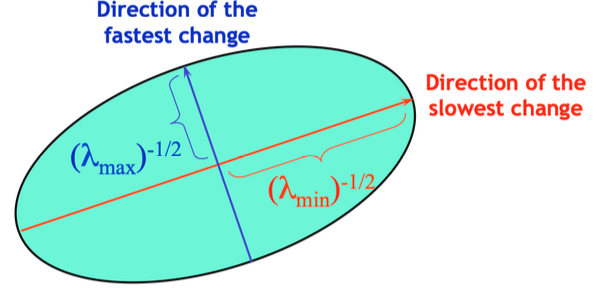
\includegraphics[width=0.8\textwidth]{figures/energy_landscope.png}
        \caption{Energy Landscape}
    \end{minipage}
    \begin{minipage}[t]{0.5\textwidth}
        \centering
        \includegraphics[width=0.9\textwidth]{figures/corner_map.png}
        \caption{特征值大小和点种类的关系}
    \end{minipage}
\end{figure}

根据这两个特征值的大小可以判断这个点是不是角点. 这个点是角点一般需要满足:

\begin{itemize}
    \item $\lambda_1, \lambda_2>b$
    \item $\frac{1}{k}<\frac{\lambda_1}{\lambda_2}<k$
\end{itemize}

一个快速的判断公式:

\begin{equation}
\begin{aligned}
\theta&=\frac 12(\lambda_1\lambda_2-\alpha(\lambda_1+\lambda_2)^2)+\frac12(\lambda_1\lambda_2-2t)\\
&=\lambda_1\lambda_2-\alpha(\lambda_1+\lambda_2)^2-t\\
&=\det(R)-\alpha\text{Trace}(R)^2-t, \text{ where } \alpha\in[0.04,0.06], t\in[0.01,0.03].
\end{aligned}
\end{equation}

当 $\theta > \tau$ 时, 则认为这个点是角点. 其中 $\tau$ 通常是一个较小的正数.


Harris Corner 对平移和图像旋转是 equivariant的,对尺度变换 (Scale) 不是 equivariant 的.

\textbf{Choices of Window Function:} 由于 Rectangle window function 不具有旋转不变性, 可以使用 Gaussian window function(Isotropic "soft" window) 代替, 即
\[
    g_\sigma(x,y)=\frac{1}{2\pi\sigma^2}\exp\left( -\frac{x^2+y^2}{2\sigma^2} \right) \implies M(x_0, y_0) = \begin{bmatrix}
        g_\sigma \ast I_x^2 & g_\sigma \ast I_xI_y \\ g_\sigma \ast I_xI_y & g_\sigma \ast I_y^2 
    \end{bmatrix}
\]
此时, (记 $g_\sigma \ast \cdot = g(\cdot)$
\begin{align*}j
    \theta(x_0, y_0) &= \det(M(x_0, y_0)) - \alpha \text{Trace}(M(x_0, y_0))^2 - t \\
    &= \left(g(I_x^2) g(I_y^2) - g(I_xI_y)^2\right) - \alpha \left(g(I_x^2) + g(I_y^2)\right)^2 - t.
\end{align*}

\textbf{In Summary:} The whole process of Harris Corner Detection is as follows:
\begin{figure}[htbp]
    \centering
    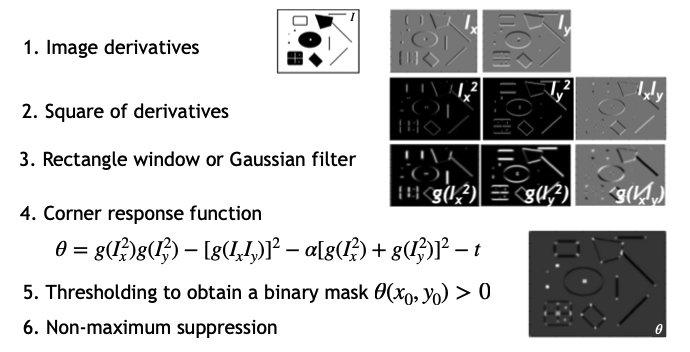
\includegraphics[width=0.8\textwidth]{figures/Harris_process.png}
    \caption{Harris Corner Detection}
\end{figure}
\subsection{equivariant V.S. invariant}
考虑 $X \in V$, 函数$F: V \to V$ 和变换 $T: V \to V$ (translation, rotation, etc.)
\begin{itemize}
    \item 等变 (equivariant): $F(TX)=T(F(x))$,对于translation和rotation是等变的. 检查 $\theta$ 即可.
    \item 不变 (invariant): $F(T(X))=F(X)$,也就是对于不同位置导出的角点还是那样,所以其实我们想要的是等变,也就是对于不同位置导出的角点做了同样的变化. 对于分类等输出较类别的问题,我们通常需要不变性.
\end{itemize}

\subsection{How to prove Harris detector is equivariant?}

只要说明角点检测函数也是equivariant即可.

角点检测函数包括了求导和卷积两个操作,显然求导是equivariant的,因为导数会随着trans和rot做相同的变化.

很有趣的是卷积也是equivariant的:当你的filter function是各向同性的,那么这个卷积就是equivariant的;但是如果是一个椭圆形的window,那这个卷积就不是equivariant的了.

\begin{figure}[htbp]
    \centering
    \includegraphics[width=0.6\textwidth]{figures/light_invariant.png}
    \caption{Illumination invariant}
\end{figure}

这个高光说明不是环境 Illumination Invariant的

\subsection{How to do NMS with corner-response-function?}

一个简单的想法:

先给出一个阈值,把所有response排序,成为一个list,从上到下按顺序把这个pixel周围的大于阈值的踢出list.
这个跟之前的NMS区别在于之前需要一条边,现在只需要一个点,那么现在比之前踢出的像素点更多.

\subsection{Scale Invariant Detectors}

Harris-Laplacian, SIFT (Lowe)